\documentclass[aspectratio=169]{beamer}

\usepackage[T1]{fontenc}
\usepackage[utf8]{inputenc}
\usepackage[english]{babel}
\usepackage{pgfplots}
\pgfplotsset{compat=newest}
\usepackage{booktabs}
\usepackage{siunitx}
\usepackage{amsmath}
\DeclareMathOperator*{\argmin}{arg\,min}

\usepackage{tikz}

\usefonttheme{professionalfonts}
\usepackage{fontspec}
\setsansfont
  [Ligatures=TeX, % recommended
   UprightFont={* Light},
   ItalicFont={* Light Italic},
   BoldFont={* Medium},
   BoldItalicFont={* Medium Italic}]
  {Neo Sans Std}
%\setromanfont{Neo Sans Std}

% Remove Figure word from caption
\setbeamertemplate{caption}{\footnotesize\raggedright\insertcaption\par}

\newcommand{\oc}{\begin{column}{.5\textwidth}}
\newcommand{\ec}{\end{column}}
\newcommand{\ocs}{\begin{columns}[c,onlytextwidth]}
\newcommand{\ecs}{\end{columns}}
\usepackage{mathtools}

\usepackage{unicode-math}
%\setmathfont{Latin Modern}

% Latin Modern
%\usepackage{lmodern}
% Verdana font type
%\usepackage{verdana}
% Helvetica
%\usepackage{helvet}
% Times (text and math)
%\usepackage{newtx, newtxmath}

\usetheme[department=elektro,showsection=true]{DTU}

\setbeamertemplate{section page}
{
\hfill \color{white} {\LARGE \insertsection}
%\par
}

\AtBeginSection[]{
\begingroup
\setbeamercolor{background canvas}{bg=dtured}
\frame[dtuwhitelogo,noframenumbering]{\sectionpage}
\endgroup
}

\title[PhD defence]{Demand Response for a Secure Power System Operation}
\subtitle{Service Specification, Validation and Verification in view of Distributed Energy Systems}
\author{Daniel Esteban Morales Bondy}
\institute{Energy Systems Operation and Management\\ Center for Electric Power and Energy \\ Technical University of Denmark \\ \vspace{1cm} \today}
\date{\today}
	
\newcommand{\tabitem}{{\color{dtured}$\bullet$} }

\begin{document}
\frame[noframenumbering]{
	\maketitle
}

\frame{
\frametitle{With support from:}
\begin{figure}
	\begin{minipage}[b]{0.7\linewidth}
	\centering
	\includegraphics[width=0.6\textwidth]{figures/iPower_Logo.eps}
	%\caption{The traditional power system, where energy flows from producer to consumer.}
	\end{minipage}
	\hspace{3cm}
	\begin{minipage}[b]{0.3\linewidth}
	\centering
	\includegraphics[width=\textwidth]{figures/PowerLab_logo.pdf}
	%\caption{The future power system includes renewable generation and advanced ICT.}
	\end{minipage}
\end{figure}
}

\frame{
	\frametitle{Outline}
	\tableofcontents
}

\section{Introduction}
\subsection*{Changes in the power system}
\frame{
	\frametitle{Energy supply must be sustainable and clean}
	\ocs
	\oc
	\ec
	\oc
	\only<1>{The world faces:
	\begin{itemize}
	\item[] Climate issues
	\item[] Health issues
	\item[] Geopolitical issues
	\end{itemize}}
	\only<2>{
	The Danish solution: 
	\begin{itemize}
	\item[]50\% of electricity generated by wind in 2020
	\item[]50\% of all energy production comes from renewable sources by 2030
	\item[]Fossil fuel independent by 2050
	\end{itemize}}
	\ec
	\ecs
}

\frame{
\frametitle{Renewable generation impacts the reliability \\ of the power system}%From production follows consumption to \\ consumption (partly) follows production
\setbeamercovered{transparent}
\begin{figure}
	\begin{minipage}[b]{0.3\linewidth}
	\centering
	\includegraphics<1>[width=\textwidth]{figures/traditional_grid_new.eps}
	\includegraphics<2->[width=\textwidth]{figures/traditional_grid_new_tr.eps}
	\caption{\uncover<1>{The traditional power system, where energy flows from producer to consumer.}}
	\end{minipage}
	\hspace{3cm}
	\begin{minipage}[b]{0.3\linewidth}
	\centering
	\includegraphics<1>[width=\textwidth]{figures/smart_grid_new_tr.eps}
	\includegraphics<2->[width=\textwidth]{figures/smart_grid_new.eps}
	\caption{\uncover<2->{The future power system includes renewable generation and advanced ICT.}}
	\end{minipage}
\end{figure}
%\begin{figure}
%
%
%\end{figure}
%
%\begin{figure}
% \hspace{2cm}
%\includegraphics[width=0.3\columnwidth]{figures/}
%\caption{}
%\end{figure}
}

\frame{
\frametitle{New sources for ancillary services are needed}
\ocs
\oc

\ec
\oc
\begin{itemize}
\item[] Ancillary services are critical
\item[] We need to rethink the operation of the system
\item[] Demand response of DERs can provide services
\end{itemize}
\ec
\ecs
}
\frame{
\frametitle{The Demand Response Aggregator \\ is a new service provider}
\begin{figure}
\centering
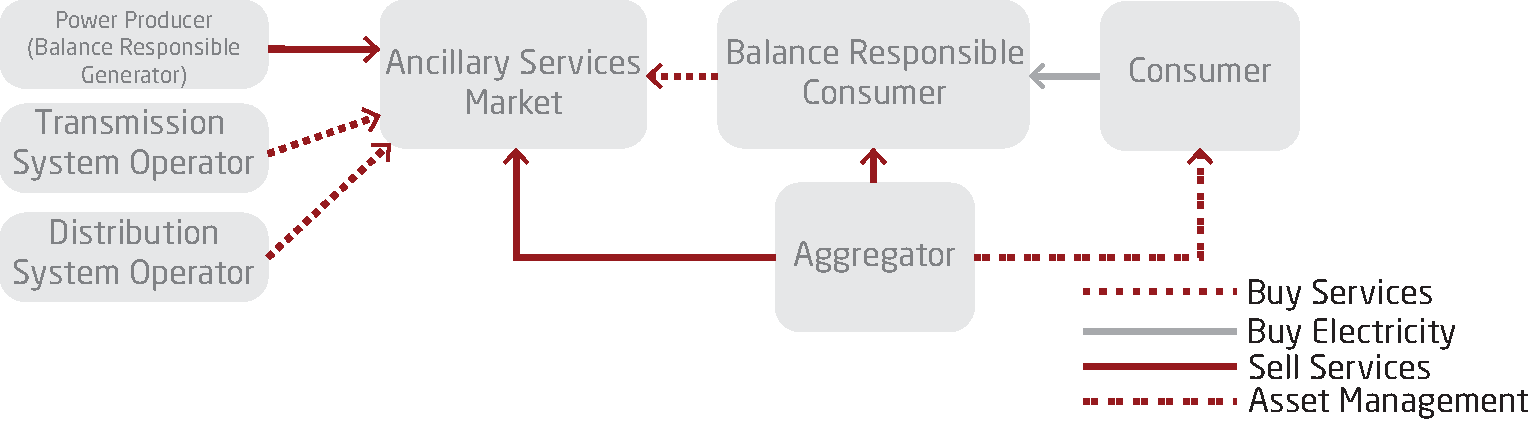
\includegraphics[width = 0.7\textwidth]{figures/market_future.eps}
\caption{A future market setup with an independent aggregator.}
\end{figure}
}

\subsection*{Problem Statement}
\frame{
\frametitle{How do we ensure aggregator reliability?}
\ocs
\oc
\begin{figure}
\centering
\includegraphics[width = 0.7\textwidth]{figures/framework3.eps}
\caption{Guiding concept behind the research.}
\end{figure}
\ec
\oc
\begin{itemize}
\item[1.-] How do we validate aggregators?
\item[2.-] Which are the service needs aggregators satisfy?
\item[3.-] How do we quantify performance in service delivery?
\end{itemize}
\ec
\ecs
}


\section{The Aggregator}
\frame{
\frametitle{A reference architecture is needed in order to\\ have a common understanding of what an aggregator is}
\ocs
	\oc
		\begin{center}
			\begin{figure}
			\includegraphics[width=\columnwidth]{figures/domains3.eps}
			\caption{The aggregator concept spreads across domains.}
			\end{figure}
		\end{center}
	\ec
	\oc
	\setlength{\partopsep}{0pt}
		A reference architecture must provide:
			\begin{itemize}
			\item[] A common lexicon and taxonomy
			\item[] Modularization and complementary context
			\item[] A common architectural vision
		\end{itemize}
	\ec
\ecs
}
\frame{
\frametitle{A reference architecture for describing the aggregator}
		\begin{center}
		\begin{figure}
		\includegraphics[width=.6\textwidth]{figures/diag_simple3.eps}
		\caption{The aggregator functional reference architecture abstracts from specific control architectures.}
		\end{figure}
		\end{center}
}

\frame{
\frametitle{Example: OpenEnergi}
\begin{center}
		\begin{figure}
		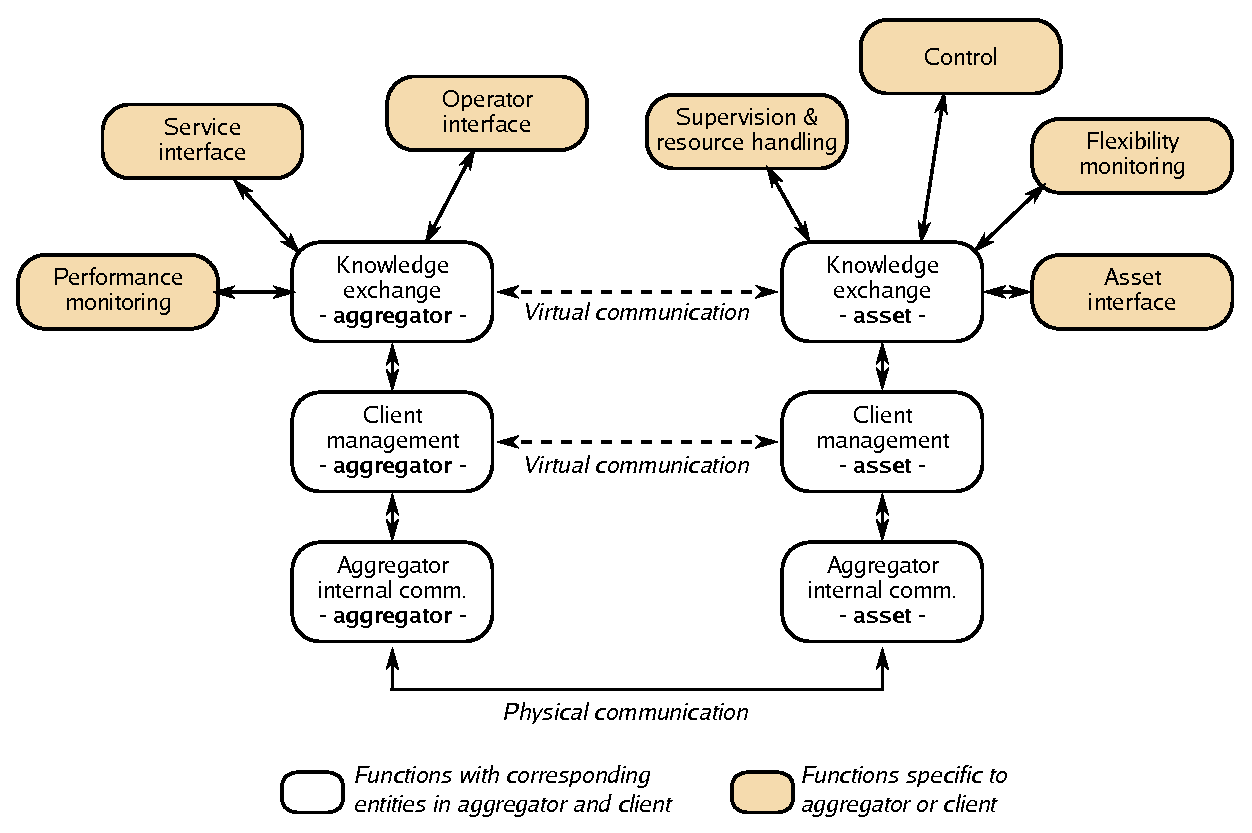
\includegraphics[width=.6\textwidth]{figures/stackdrawing_openenergi.eps}
		\caption{OpenEnergi is a fully distributed aggregator.}
		\end{figure}
		\end{center}

}

\frame{
\frametitle{Contributions}
\ocs
\oc
\ec
\oc
A candidate reference architecture with the purpose of:
\begin{itemize}
\item[] Defining a standard lexicon
\item[] Identifying the required functionality for an effective aggregator
\end{itemize}
\ec
\ecs

}

\section{How do we validate aggregators?}



\frame{
\frametitle{Current procedures are insufficient due to the \\ differences between aggregators and generators}
%\setbeamercovered{transparent}
\ocs
	\oc
		\begin{center}
			\begin{figure}
			\includegraphics[width=\textwidth]{figures/swissresponse.eps}
			\caption{Prequalification test in SwissGrid}
			\end{figure}
		\end{center}
	\ec
	\oc
	\setlength{\partopsep}{0pt}
		\only<1>{Current procedure:}
		\only<2->{New procedure:}
		\only<1>{
		\begin{itemize}
			\item[] Documentation
			\item[] Prequalification test
		\end{itemize}
		}
		\only<2->{
		\begin{itemize}
			\item[] Documentation
			\item[] Validation through Simulation
			\item[] Prequalification test \& Monitoring
		\end{itemize}
		}
	\ec
\ecs
}

\frame{
\frametitle{Aggregators are essentialy different from generators}
\ocs
	\oc
		\begin{center}
			\begin{figure}
			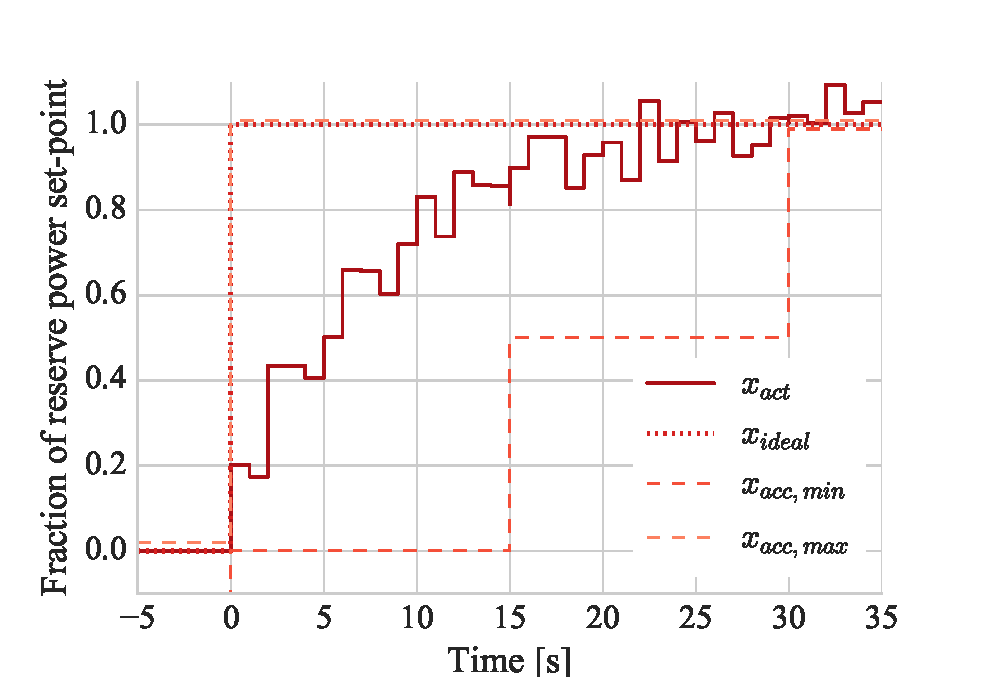
\includegraphics[width=0.8\textwidth]{figures/primfreqresp2.eps}
			\caption{Example of an aggregator response to step input.}
			\end{figure}
		\end{center}
	\ec
	\oc
	\setlength{\partopsep}{0pt}
		\begin{itemize}
			\item[] Heterogeneous in composition: not necessarily described through analytical methods
			\item[] Geograghically distributed: no single point of measurement
			\item[] Different failure modes: reliability must be evaluated differently
			\item[] Architectures vary: new operating conditions are relevant
		\end{itemize}
	\ec
\ecs
}

\frame{
\frametitle{Validation of aggregators must rely on \\ statistical Design of Experiments}
\ocs
	\oc
		%Simulation through validation:
		\begin{center}
			\begin{figure}
			\includegraphics[width=0.7\textwidth]{figures/framework.eps}
			\caption{Conceptual validation framework}
			\end{figure}
		\end{center}
	\ec
	\oc
	\setlength{\partopsep}{0pt}
			\begin{enumerate}
			\item Documentation of portfolio
			\item Identification of service requirements
			\item Identification of normal operation of the aggregator
			\item Definition of operation scenarios
			\item Tests are carried out according to an experiment design
			\begin{itemize}
			\item[] Which treatments? How many replications? How will each factor vary between treatment?
			\end{itemize}
			\item Performance evaluation
		\end{enumerate}
	\ec
\ecs
}
\frame{
\frametitle{Example: Direct control of house heating}
 
\begin{figure}
	\begin{minipage}[b]{0.45\linewidth}
	\centering
	\includegraphics[width=\columnwidth]{figures/agg_power_ctrl_100SH_0STATIC_05PCT_REDUCTIONcrop.eps}\\
	\includegraphics[width=\columnwidth]{figures/agg_power_ctrl_70SH_30STATIC_05PCT_REDUCTIONcrop.eps}%
	\caption{Aggregator test at full functionality and at expected minimum functionality.}
	\end{minipage}
	\hspace{1cm}
	\begin{minipage}[b]{0.45\linewidth}
	\centering
	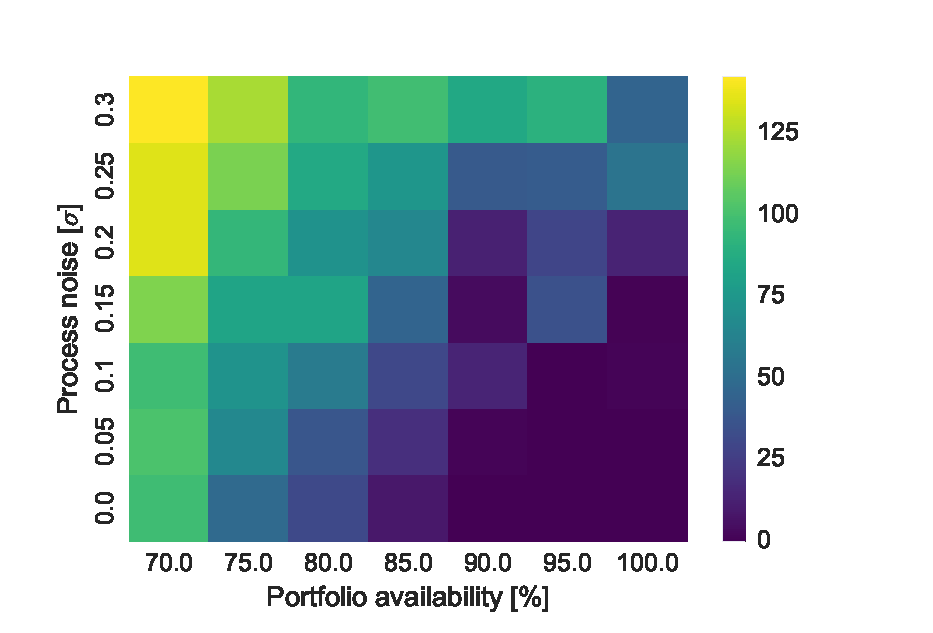
\includegraphics[width=\columnwidth]{figures/heatmap.eps}%
	\caption{Fractional factorial test of the aggregator.}
	\end{minipage}
\end{figure} 
}

\frame{
\frametitle{Contributions}
\ocs
\oc
\ec
\oc
Expansion of traditional methods for prequalification:
\begin{itemize}
\item[] Application of Design of Experiments concepts to the statistical validation of aggregators
\end{itemize}
\ec
\ecs
}


%{\setbeamercolor{background canvas}{bg=black}
%\frame[dtuwhitelogo]{some text}}
\section{Which are the service needs aggregators satisfy?}
\frame{
\frametitle{Aggregators can supply existing services \\ as well as new services}
\ocs
\oc
\ec
\oc
\begin{itemize}
\item[TSO:] Ancillary services
\item[DSO:] Voltage control and congestion management
\item[BRP:] Portfolio Balancing
\item[Consumers:] Asset Management Service 
\end{itemize}
\ec
\ecs
}


\frame{
\frametitle{Current regulatory framework is a barrier \\ for aggregation and demand response in many countries}
\setbeamercovered{transparent}
\ocs
\oc
\ec
\oc
\begin{itemize}
\item<-2>[] Temporal requirements
\item<-1>[] Resource tuning requirements
\item<-1>[] Market requirements
\end{itemize}
\ec
\ecs
}

\frame{
\frametitle{Services should be modeled \\ only in terms of performance}
\begin{enumerate}
  \item Identify the parameters required for assessing the service delivery ($n_{del}$)
  \item Identify the relation between system parameters ($n_{k}$) and required service
  \item Quantify the physical volume of the service
  \item Characterize the boundaries of service delivery
  \item Develop mappings for ideal and acceptable service provision, $h_{id}:\mathbb{R}^{n_{k}}\rightarrow \mathbb{R}^{n_{id}}$, and  $h_{ac}:\mathbb{R}^{n_{k}}\times\mathbb{R}^{n_{id}}\rightarrow \mathbb{R}^{n_{ac}}$ 
  \item Establish a measure for acceptable aggregation for the measurement of service delivery $h_{m}:\mathbb{R}^{n_{m}}\rightarrow \mathbb{R}^{n_{del}}$, and the service error $h_{e}:\mathbb{R}^{n_{id}}\times\mathbb{R}^{n_{del}}\rightarrow \mathbb{R}$
\end{enumerate}
}
\frame{
\frametitle{We identify three generic model patterns}
\ocs
\oc
\ec
\oc
\begin{itemize}
\item[] Reference tracking service
\item[] Band service
\item[] Cap service
\end{itemize}
\ec
\ecs
}
\frame{
\frametitle{Reference tracking}
\ocs
\oc
	\begin{center}
	\begin{figure}
	\includegraphics[width=0.7\textwidth]{figures/tracking_error2.eps}
	\caption{$h_{e}$ for reference tracking services}
	\end{figure}
	\end{center}
\ec
\oc
\begin{equation*}
e(t) = x_{del}(t) - x_{ideal}(t),
\end{equation*}
\begin{align*}
&x_{acc,max}(t) = x_{ideal}(t) + c_{max}(t), \\
&x_{acc,min}(t) = x_{ideal}(t) - c_{min}(t),
\end{align*}
\ec
\ecs
}

\frame{
\frametitle{Band service}
\ocs
\oc
	\begin{center}
	\begin{figure}
	\includegraphics[width=0.7\textwidth]{figures/band_error2.eps}
	\caption{$h_{e}$ for reference band services}
	\end{figure}
	\end{center}
\ec
\oc
\begin{equation*}
e(t)=
\begin{cases}
x_{del}(t) - x_{min}(t) , \quad x_{del}(t) < x_{min}(t)  \\
0, \qquad x_{min}(t) \leq x_{del}(t) \leq x_{max}(t) \\
x_{del}(t) - x_{max}(t), \quad  x_{del}(t)  > x_{max}(t)  
\end{cases}
\end{equation*}
\begin{align*}
&x_{acc,max}(t) = x_{max}(t) + c_{max}(t), \\
&x_{acc,min}(t) = x_{min}(t) - c_{min}(t)
\end{align*}
\ec
\ecs
}
\frame{
\frametitle{Cap service}
\ocs
\oc
	\begin{center}
	\begin{figure}
	\includegraphics[width=0.7\textwidth]{figures/cap_error2.eps}
	\caption{$h_{e}$ for cap services}
	\end{figure}
	\end{center}
\ec
\oc
\begin{equation*}
e(t)=
\begin{cases}
x_{del}(t)-x_{max}(t), & x_{del}(t) > x_{max}(t) \\
0, & x_{del}(t) \leq x_{max}(t)
\end{cases}
\end{equation*}
\begin{equation*}
x_{acc,max} = x_{max}(t) + c_{max}(t)
\end{equation*}
\ec
\ecs
}

\frame{
\frametitle{Ancillary service reserves are contracted based \\ on the least common denominator for performance}
\begin{center}
\begin{figure}
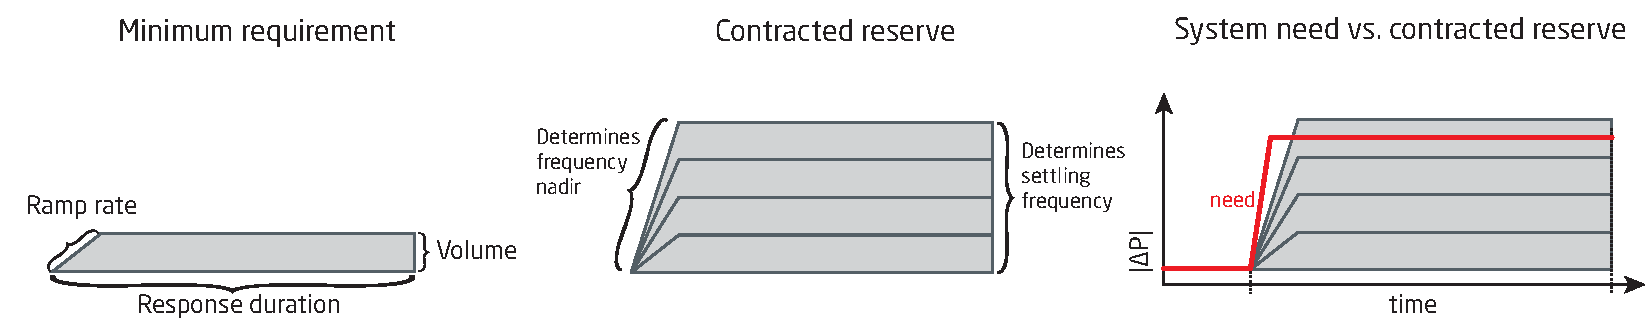
\includegraphics[width=0.95\textwidth]{figures/traditional_reserve_dim.pdf}
\caption{Traditional reserve procurement is based upon offline static analysis.}
\end{figure}
\end{center}
}

\frame{
\frametitle{New resources have different properties \\ that are beneficial to the system}
\begin{center}
\begin{figure}
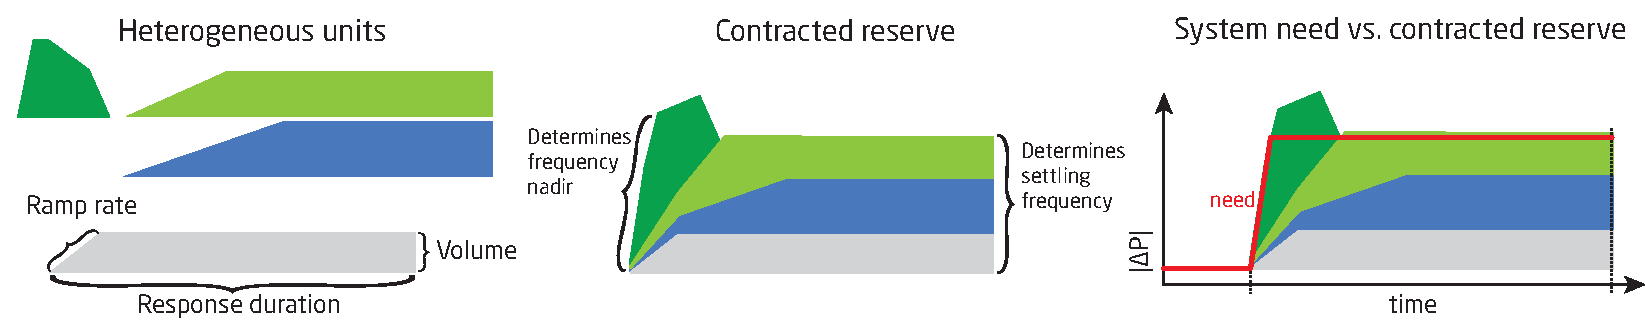
\includegraphics[width=0.95\textwidth]{figures/new_reserve_dim.pdf}
\caption{Modern reserve procurement should take the different resource capabilities into account.}
\end{figure}
\end{center}
}

\frame{
\frametitle{Ancillary service requirements need to be \\ redefined for technology agnostic resources}
\ocs
\oc
\ec
\oc
The overall approach to restructuring ancillary services:
\begin{enumerate}
\item Formulate an ideal response
\item Parametrize the ancillary service bid
\item Calculate the capability value of a unit according to its parameters
\item Clear all units under a generalized single clearing-price auction
\item Performance-based remuneration
\end{enumerate}
\ec
\ecs
}

\frame{
\frametitle{Example: Frequency Containment Reserve \\ SYSLAB experiment}
\ocs
\oc
\begin{center}
\begin{figure}
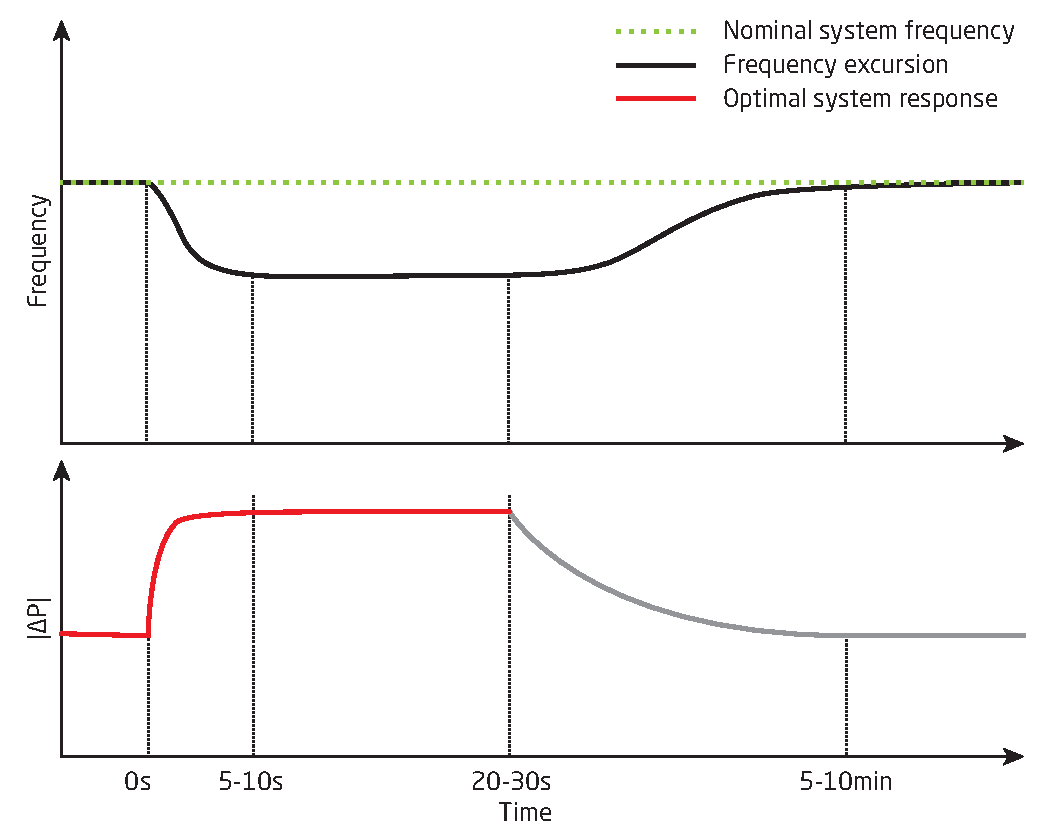
\includegraphics[width=0.7\textwidth]{figures/primary_frequency_control_ideal.eps}
\caption{The desired ideal response depends on the inertia of the system.}
\end{figure}
\end{center}
\ec
\oc
Required ideal response:
\begin{equation*}
V_{TSO}=f\left(\tau^r_{TSO},\tau^d_{TSO},C_{TSO}\right)
\end{equation*}

Bids from service providers:
\begin{equation*}
\text{Bid} = \left(  \tau^r_i,\tau^d_i,C_i, P^\mathtt{bid}_i\right)
\end{equation*}
\ec
\ecs
}

\frame{
\frametitle{Example: Frequency Containment Reserve \\ SYSLAB experiment (continued)}
Capability value: $$	\kappa_i = \alpha_1 \frac{\tau_{r,0}}{\max({\tau_{r,0},\tau_{r,i})}} + \alpha_2  \frac{\min(\tau_{d,0},\tau_{d,i})}{\tau_{d,0}} + \alpha_3 \frac{V_i}{V_{tot}}, \quad \forall \, i \in \Omega,\sum_{i} \alpha_i = 1 $$ 
Market clearing:
\begin{align*}
      \Omega^\mathtt{acc} = \argmin_{\Omega \in \mathcal P(\Omega^{rec})}  \sum_{i\in \Omega}& { \kappa_i P^\mathtt{clear} }   \\
      \mathtt{s.t.}  \sum_{i\in \Omega} \left(1-\eta_i \right) V_{i} & \geq V_{TSO}\\
       P^\mathtt{clear} &= \max P^\mathtt{bid}_i\\
       \epsilon_{i} & \leq \epsilon_{max}
\end{align*}
Performance based remuneration:
$$ P^\mathtt{rem}_i = \left( 1 - \eta_i\right) \kappa_i  P^\mathtt{clear} V_i \qquad \forall i \in \Omega^\mathtt{acc} $$
}

\frame{
\frametitle{Example: Frequency Containment Reserve\\ SYSLAB experiment results}
\begin{figure}
	\begin{minipage}[b]{0.45\linewidth}
	\centering
	\includegraphics[width=\columnwidth]{figures/MeritOrder}
	\caption{Clearing according to merit order.}
	\end{minipage}
	\hspace{1cm}
	\begin{minipage}[b]{0.45\linewidth}
	\centering
	\includegraphics[width=\columnwidth]{figures/newClearing}%
	\caption{Clearing according to capability value.}
	\end{minipage}
\end{figure} 
}

\frame{
\frametitle{Contributions}
\ocs
\oc
\ec
\oc
Enabled the delivery of services from aggregators by:
\begin{itemize}
\item[] General method for modeling services
\item[] Redefinition of ancillary service requirements 
\end{itemize}
\ec
\ecs
}
\section{How do we quantify performance in service delivery?}
\frame{
\frametitle{Service Performance Assessment is useful \\ at various stages of service delivery}
\ocs
\oc
\ec
\oc
\begin{itemize}
\item[] Prequalification process
\item[] Monitoring during delivery
\item[] Verification post-delivery
\item[] Financial settlement
\end{itemize}
\ec
\ecs
}

\frame{
\frametitle{Performance indices inspired from process control:\\ Control Performance Assessment}
\ocs
\oc
\ec
\oc
Desired indices:
\begin{align*}
    \text{[SPI]:} \quad & \eta = f_P(x_{del},\mathbf{x}_{acc},t), \quad \eta \in [0,1]\\
    \text{[SVI]:} \quad & \epsilon = f_R(x_{del},\mathbf{x}_{acc},t)
\end{align*}
\ec
\ecs
}
\frame{
\frametitle{Quality of Service is defined  \\ by the service error models}
\ocs
\oc
\ec
\oc
Quality of service defined by:
$$ QoS(t) = e(t) C_n (t)$$

Scaling factor defined by:
\begin{equation*}
C_{n}(t) = 
\begin{cases}
\frac{1}{x_{acc,max}(t) - x_{max}(t)}, & e(t) \geq 0 \\
\frac{1}{x_{acc,min}(t) - x_{min}(t)}, & e(t) < 0
\end{cases}
\end{equation*}
\ec
\ecs
}
\frame{
\frametitle{Visual representation of QoS}
\begin{figure}
	\begin{minipage}[b]{0.3\linewidth}
	\centering
	\includegraphics[width=\columnwidth]{figures/tracking_error2}\\
	\includegraphics[width=\columnwidth]{figures/tracking_error3}
	\caption{QoS of reference tracking services.}
	\end{minipage}
	\hspace{0.5cm}
	\begin{minipage}[b]{0.3\linewidth}
	\centering
	\includegraphics[width=\columnwidth]{figures/band_error2}\\
	\includegraphics[width=\columnwidth]{figures/band_error3}
	\caption{QoS of band services.}
	\end{minipage}
	\hspace{0.5cm}
	\begin{minipage}[b]{0.3\linewidth}
	\centering
	\includegraphics[width=\columnwidth]{figures/cap_error2}\\
	\includegraphics[width=\columnwidth]{figures/cap_error3}
	\caption{QoS of cap services.}
	\end{minipage}
\end{figure} 
}
\frame{
\frametitle{The Service Performance Index evaluates \\ performance within the acceptable bounds}
\ocs
\begin{column}{.4\textwidth}
\ec
\begin{column}{.6\textwidth}
We truncate the measured error:
\begin{align*}
	QoS^{AS}(t) = \begin{cases} QoS^{AS}_{meas}(t) ,\quad &\forall QoS^{AS}_{meas}(t) \leq 1, \forall t\\
	1, \quad &\forall QoS^{AS}_{meas}(t) > 1, \forall t
	\end{cases}
\end{align*}

We define the SPI as:
\begin{equation*}
\eta^{AS} = \sqrt{\frac{\sum^{N}_{t=0} \left( {QoS^{AS}_{t}}^{2} \right)}{t_N}} 
\end{equation*}
\ec
\ecs
}
\frame{
\frametitle{The Service Verification Index evaluates \\ the non-delivery of service}
\ocs
\begin{column}{.4\textwidth}
\ec
\begin{column}{.6\textwidth}
We only measure error outside the acceptable bounds:
\begin{align*}
	ND^{AS}(t) = \begin{cases} QoS^{AS}_{meas}(t) - 1,\quad &\forall QoS^{AS}_{meas}(t) > 1, \forall t\\
	0, \quad &\forall QoS^{AS}(t) \leq 1, \forall t
	\end{cases}
\end{align*}

We define the SVI as:
\begin{equation}
\epsilon^{AS} = \sqrt{\frac{\sum^{N}_{t=0} \left( {ND^{AS}_{t}}^{2} \right)}{t_N}}
\end{equation}
\ec
\ecs
}

\frame{
\frametitle{Contributions}
\ocs
\oc
\ec
\oc
We enable evaluation of aggregators by applying concepts from process control:
\begin{itemize}
\item[] Service Performance Index
\item[] Service Verification Index
\end{itemize}
\ec
\ecs
}
%{
%\setbeamercolor{background canvas}{bg=black} % Background color
%	\frame[dtuwhitelogo]{
%		\frametitle{Hello Blackness}
%		Here is another frame style!
%	}
%}

\section{Conclusion}
\frame{
\frametitle{New operation methods must be developed \\ in order to cope with fluctuating renewable resources}
\ocs
\oc
	\begin{center}
	\begin{figure}
	\includegraphics[width=0.7\textwidth]{figures/framework2.eps}
	\caption{Conceptual framework for aggregator validation}
	\end{figure}
	\end{center}
\ec
\oc
\begin{itemize}
\item[] Service Specification:
\begin{itemize}
\item Procedure for generic service modeling
\item Redefinition of ancillary service requirements
\end{itemize}
\item[] Aggregator prequalification:
\begin{itemize}
\item Documentation through functional reference architecture
\item Application of DoE to aggregator validation
\end{itemize}
\item[] Service Verification:
\begin{itemize}
\item Application of CPA concepts to the verification of service delivery
\item Service Performance Index
\item Service Verification Index
\end{itemize}
\end{itemize}
\ec
\ecs
}

\frame{
\frametitle{Further work}
\ocs
\oc
\ec
\oc
\begin{itemize}
\item[] Operation scenario descriptions
\item[] How do you validate simulations with physical tests
\item[] How do you map measurement aggregation to service delivery: $h_n$
\end{itemize}
\ec
\ecs
}



%================================================
%===  Define the contact details
\newcommand\contactTable{ %
  \begin{tabular}{lr}
    \multicolumn{2}{l}{Daniel Esteban Morales Bondy} \\ 
    \multicolumn{2}{l}{CEE, Technical University of Denmark (DTU)} \\ \midrule
    Building 776, Room 05    & bondy@elektro.dtu.dk. \\
    4000 Roskilde, Denmark & +45 30139930
  \end{tabular}
}%

\frame[dtuwhitelogo, bgfilename=figures/risoe.eps]{ % 
  \begin{tikzpicture}[remember picture,overlay]
    \node[fill=black, fill opacity=0.9, 
          text=white, text opacity=1.0,
          rounded corners=5pt, 
          font=\scriptsize] at (current page.center) {\contactTable};
  \end{tikzpicture}
}

\end{document}